\definecolor{c1}{rgb}{0 0.4470 0.7410}
\definecolor{c2}{rgb}{0.8500 0.3250 0.0980}
\definecolor{c3}{rgb}{0.9290 0.6940 0.1250}
\definecolor{c4}{rgb}{0.4940 0.1840 0.5560}
\definecolor{c5}{rgb}{0.4660 0.6740 0.1880}
\definecolor{c6}{rgb}{0.3010 0.7450 0.9330}
\definecolor{c7}{RGB}{251,180,185}
\definecolor{c8}{RGB}{247,104,161}
\definecolor{c9}{RGB}{255,0,255}
\definecolor{g}{RGB}{44,162,95}
\definecolor{r}{RGB}{227,74,51}

% GNUPLOT: LaTeX picture with Postscript
\begingroup
  \makeatletter
  \providecommand\color[2][]{%
    \GenericError{(gnuplot) \space\space\space\@spaces}{%
      Package color not loaded in conjunction with
      terminal option `colourtext'%
    }{See the gnuplot documentation for explanation.%
    }{Either use 'blacktext' in gnuplot or load the package
      color.sty in LaTeX.}%
    \renewcommand\color[2][]{}%
  }%
  \providecommand\includegraphics[2][]{%
    \GenericError{(gnuplot) \space\space\space\@spaces}{%
      Package graphicx or graphics not loaded%
    }{See the gnuplot documentation for explanation.%
    }{The gnuplot epslatex terminal needs graphicx.sty or graphics.sty.}%
    \renewcommand\includegraphics[2][]{}%
  }%
  \providecommand\rotatebox[2]{#2}%
  \@ifundefined{ifGPcolor}{%
    \newif\ifGPcolor
    \GPcolorfalse
  }{}%
  \@ifundefined{ifGPblacktext}{%
    \newif\ifGPblacktext
    \GPblacktexttrue
  }{}%
  % define a \g@addto@macro without @ in the name:
  \let\gplgaddtomacro\g@addto@macro
  % define empty templates for all commands taking text:
  \gdef\gplfronttext{}%
  \gdef\gplfronttext{}%
  \makeatother
  \ifGPblacktext
    % no textcolor at all
    \def\colorrgb#1{}%
    \def\colorgray#1{}%
  \else
    % gray or color?
    \ifGPcolor
      \def\colorrgb#1{\color[rgb]{#1}}%
      \def\colorgray#1{\color[gray]{#1}}%
      \expandafter\def\csname LTw\endcsname{\color{white}}%
      \expandafter\def\csname LTb\endcsname{\color{black}}%
      \expandafter\def\csname LTa\endcsname{\color{black}}%
      \expandafter\def\csname LT0\endcsname{\color[rgb]{1,0,0}}%
      \expandafter\def\csname LT1\endcsname{\color[rgb]{0,1,0}}%
      \expandafter\def\csname LT2\endcsname{\color[rgb]{0,0,1}}%
      \expandafter\def\csname LT3\endcsname{\color[rgb]{1,0,1}}%
      \expandafter\def\csname LT4\endcsname{\color[rgb]{0,1,1}}%
      \expandafter\def\csname LT5\endcsname{\color[rgb]{1,1,0}}%
      \expandafter\def\csname LT6\endcsname{\color[rgb]{0,0,0}}%
      \expandafter\def\csname LT7\endcsname{\color[rgb]{1,0.3,0}}%
      \expandafter\def\csname LT8\endcsname{\color[rgb]{0.5,0.5,0.5}}%
    \else
      % gray
      \def\colorrgb#1{\color{black}}%
      \def\colorgray#1{\color[gray]{#1}}%
      \expandafter\def\csname LTw\endcsname{\color{white}}%
      \expandafter\def\csname LTb\endcsname{\color{black}}%
      \expandafter\def\csname LTa\endcsname{\color{black}}%
      \expandafter\def\csname LT0\endcsname{\color{black}}%
      \expandafter\def\csname LT1\endcsname{\color{black}}%
      \expandafter\def\csname LT2\endcsname{\color{black}}%
      \expandafter\def\csname LT3\endcsname{\color{black}}%
      \expandafter\def\csname LT4\endcsname{\color{black}}%
      \expandafter\def\csname LT5\endcsname{\color{black}}%
      \expandafter\def\csname LT6\endcsname{\color{black}}%
      \expandafter\def\csname LT7\endcsname{\color{black}}%
      \expandafter\def\csname LT8\endcsname{\color{black}}%
    \fi
  \fi
    \setlength{\unitlength}{0.0500bp}%
    \ifx\gptboxheight\undefined%
      \newlength{\gptboxheight}%
      \newlength{\gptboxwidth}%
      \newsavebox{\gptboxtext}%
    \fi%
    \setlength{\fboxrule}{0.5pt}%
    \setlength{\fboxsep}{1pt}%

    \hspace{1.8cm}
\begin{picture}(8000.00,7000.00)%
    \gplgaddtomacro\gplfronttext{%
      \colorrgb{0.15,0.15,0.15}%
      \put(-52,5734){\makebox(0,0)[r]{\strut{}\small $1.0$$\cdot$$10^5$}}%
      \colorrgb{0.15,0.15,0.15}%
      \put(-52,6331){\makebox(0,0)[r]{\strut{}\small $1.5$$\cdot$$10^5$}}%
      \colorrgb{0.15,0.15,0.15}%
      \put(-52,6929){\makebox(0,0)[r]{\strut{}\small $2.0$$\cdot$$10^5$}}%
      \colorrgb{0.15,0.15,0.15}%
      \put(80,5394){\makebox(0,0){\strut{}}}%
      \colorrgb{0.15,0.15,0.15}%
      \put(1328,5394){\makebox(0,0){\strut{}}}%
      \colorrgb{0.15,0.15,0.15}%
      \put(2159,5394){\makebox(0,0){\strut{}}}%
      \colorrgb{0.15,0.15,0.15}%
      \put(2867,5394){\makebox(0,0){\strut{}}}%
    }%
    \gplgaddtomacro\gplfronttext{%
      \colorrgb{0.00,0.00,0.00}%
      \put(1639,7149){\makebox(0,0){\strut{}{\color{g}{$\|e(\bm{p}, \hat{\bm{p}}^\prime)\|_2 < \|e(\bm{p}, \hat{\bm{p}})\|_2$}}}}%
      \put(6359,7149){\makebox(0,0){\strut{}{\color{r}{$\|e(\bm{p}, \hat{\bm{p}}^\prime)\|_2 \geq \|e(\bm{p}, \hat{\bm{p}})\|_2$}}}}%

      \put(-400,7800){\makebox(0,0){\strut{}{\color{c1}{\rule[0.6mm]{0.5cm}{0.5mm}}}\small PLICP}}
      \put(600,7800){\makebox(0,0){\strut{}{\color{c2}{\rule[0.6mm]{0.5cm}{0.5mm}}}\small NDT}}
      \put(1600,7800){\makebox(0,0){\strut{}{\color{c3}{\rule[0.6mm]{0.5cm}{0.5mm}}}\small FastGICP}}
      \put(3000,7800){\makebox(0,0){\strut{}{\color{c4}{\rule[0.6mm]{0.5cm}{0.5mm}}}\small FastVGICP}}
      \put(4400,7800){\makebox(0,0){\strut{}{\color{c5}{\rule[0.6mm]{0.5cm}{0.5mm}}}\small NDT-PSO}}
      \put(5700,7800){\makebox(0,0){\strut{}{\color{c6}{\rule[0.6mm]{0.5cm}{0.5mm}}}\small TEASER}}
      \put(6600,7800){\makebox(0,0){\strut{}{\color{c7}{\rule[0.6mm]{0.5cm}{0.5mm}}}\small x1}}
      \put(7200,7800){\makebox(0,0){\strut{}{\color{c8}{\rule[0.6mm]{0.5cm}{0.5mm}}}\small uf}}
      \put(7800,7800){\makebox(0,0){\strut{}{\color{c9}{\rule[0.6mm]{0.5cm}{0.5mm}}}\small fm}}


      \put(-1542,6271){\rotatebox{90}{\makebox(0,0){\strut{}\small $\sigma_R = 0.01$ m}}}%
      \put(-1542,4885){\rotatebox{90}{\makebox(0,0){\strut{}\small $\sigma_R = 0.03$ m}}}%
      \put(-1542,3499){\rotatebox{90}{\makebox(0,0){\strut{}\small $\sigma_R = 0.05$ m}}}%
      \put(-1542,2113){\rotatebox{90}{\makebox(0,0){\strut{}\small $\sigma_R = 0.10$ m}}}%
      \put(-1542,727){\rotatebox{90}{\makebox(0,0) {\strut{}\small $\sigma_R = 0.20$ m}}}%

      \put(-942,3499){\rotatebox{90}{\makebox(0,0){\strut{}$-\sum \|e(\bm{p},\hat{\bm{p}}_i^\prime)\|_2-\|e(\bm{p},\hat{\bm{p}}_i)\|_2$}}}%
      \put(3999,3499){\rotatebox{90}{\makebox(0,0){\strut{}$+\sum \|e(\bm{p},\hat{\bm{p}}_i^\prime)\|_2-\|e(\bm{p},\hat{\bm{p}}_i)\|_2$}}}%
      \put(3999,8200){\makebox(0,0){\strut{}$\sigma_{\bm{M}} = 0.05$ m}}
    }%
    \gplgaddtomacro\gplfronttext{%
      \colorrgb{0.15,0.15,0.15}%
      \put(-52,4348){\makebox(0,0)[r]{\strut{}\small $1.0$$\cdot$$10^5$}}%
      \colorrgb{0.15,0.15,0.15}%
      \put(-52,4945){\makebox(0,0)[r]{\strut{}\small $1.5$$\cdot$$10^5$}}%
      \colorrgb{0.15,0.15,0.15}%
      \put(-52,5543){\makebox(0,0)[r]{\strut{}\small $2.0$$\cdot$$10^5$}}%
      \colorrgb{0.15,0.15,0.15}%
      \put(80,4008){\makebox(0,0){\strut{}}}%
      \colorrgb{0.15,0.15,0.15}%
      \put(1328,4008){\makebox(0,0){\strut{}}}%
      \colorrgb{0.15,0.15,0.15}%
      \put(2159,4008){\makebox(0,0){\strut{}}}%
      \colorrgb{0.15,0.15,0.15}%
      \put(2867,4008){\makebox(0,0){\strut{}}}%
    }%
    \gplgaddtomacro\gplfronttext{%
    }%
    \gplgaddtomacro\gplfronttext{%
      \colorrgb{0.15,0.15,0.15}%
      \put(-52,2962){\makebox(0,0)[r]{\strut{}\small $1.0$$\cdot$$10^5$}}%
      \colorrgb{0.15,0.15,0.15}%
      \put(-52,3559){\makebox(0,0)[r]{\strut{}\small $1.5$$\cdot$$10^5$}}%
      \colorrgb{0.15,0.15,0.15}%
      \put(-52,4157){\makebox(0,0)[r]{\strut{}\small $2.0$$\cdot$$10^5$}}%
      \colorrgb{0.15,0.15,0.15}%
      \put(80,2622){\makebox(0,0){\strut{}}}%
      \colorrgb{0.15,0.15,0.15}%
      \put(1328,2622){\makebox(0,0){\strut{}}}%
      \colorrgb{0.15,0.15,0.15}%
      \put(2159,2622){\makebox(0,0){\strut{}}}%
      \colorrgb{0.15,0.15,0.15}%
      \put(2867,2622){\makebox(0,0){\strut{}}}%
    }%
    \gplgaddtomacro\gplfronttext{%
      \colorrgb{0.15,0.15,0.15}%
    }%
    \gplgaddtomacro\gplfronttext{%
      \colorrgb{0.15,0.15,0.15}%
      \put(-52,1576){\makebox(0,0)[r]{\strut{}\small $1.0$$\cdot$$10^5$}}%
      \colorrgb{0.15,0.15,0.15}%
      \put(-52,2173){\makebox(0,0)[r]{\strut{}\small $1.5$$\cdot$$10^5$}}%
      \colorrgb{0.15,0.15,0.15}%
      \put(-52,2771){\makebox(0,0)[r]{\strut{}\small $2.0$$\cdot$$10^5$}}%
      \colorrgb{0.15,0.15,0.15}%
      \put(80,1236){\makebox(0,0){\strut{}}}%
      \colorrgb{0.15,0.15,0.15}%
      \put(1328,1236){\makebox(0,0){\strut{}}}%
      \colorrgb{0.15,0.15,0.15}%
      \put(2159,1236){\makebox(0,0){\strut{}}}%
      \colorrgb{0.15,0.15,0.15}%
      \put(2867,1236){\makebox(0,0){\strut{}}}%
    }%
    \gplgaddtomacro\gplfronttext{%
    }%
    \gplgaddtomacro\gplfronttext{%
      \colorrgb{0.15,0.15,0.15}%
      \put(-52,190){\makebox(0,0)[r]{\strut{}\small $1.0$$\cdot$$10^5$}}%
      \colorrgb{0.15,0.15,0.15}%
      \put(-52,787){\makebox(0,0)[r]{\strut{}\small $1.5$$\cdot$$10^5$}}%
      \colorrgb{0.15,0.15,0.15}%
      \put(-52,1385){\makebox(0,0)[r]{\strut{}\small $2.0$$\cdot$$10^5$}}%
      \colorrgb{0.15,0.15,0.15}%
      \put(80,-150){\makebox(0,0){\strut{}\small $3.2$$\cdot$$10^5$}}%
      \colorrgb{0.15,0.15,0.15}%
      \put(1328,-150){\makebox(0,0){\strut{}\small $3.8$$\cdot$$10^5$}}%
      \colorrgb{0.15,0.15,0.15}%
      \put(2159,-150){\makebox(0,0){\strut{}\small $4.2$$\cdot$$10^5$}}%
      \colorrgb{0.15,0.15,0.15}%
      \put(2867,-150){\makebox(0,0){\strut{}\small $E$$\cdot$$|D|$}}%
    }%
    \gplgaddtomacro\gplfronttext{%
      \colorrgb{0.15,0.15,0.15}%
      \put(1639,-480){\makebox(0,0){\strut{}$|\{\hat{\bm{p}}_{i}^\prime\}| : \|e(\bm{p}, \hat{\bm{p}}_i^\prime)\|_2 < \|e(\bm{p}, \hat{\bm{p}}_i)\|_2$}}%
    }%
    \gplgaddtomacro\gplfronttext{%
      \colorrgb{0.15,0.15,0.15}%
      \put(4668,5614){\makebox(0,0)[r]{\strut{}\small $10^{+2}$}}%
      \colorrgb{0.15,0.15,0.15}%
      \put(4668,6174){\makebox(0,0)[r]{\strut{}\small $10^{+4}$}}%
      \colorrgb{0.15,0.15,0.15}%
      \put(4668,6733){\makebox(0,0)[r]{\strut{}\small $10^{+6}$}}%
      \colorrgb{0.15,0.15,0.15}%
      \put(4800,5394){\makebox(0,0){\strut{}}}%
      \colorrgb{0.15,0.15,0.15}%
      \put(5974,5394){\makebox(0,0){\strut{}}}%
      \colorrgb{0.15,0.15,0.15}%
      \put(7148,5394){\makebox(0,0){\strut{}}}%
      \colorrgb{0.15,0.15,0.15}%
      \put(7919,5394){\makebox(0,0){\strut{}}}%
    }%
    \gplgaddtomacro\gplfronttext{%
      \colorrgb{0.00,0.00,0.00}%
    }%
    \gplgaddtomacro\gplfronttext{%
      \colorrgb{0.15,0.15,0.15}%
      \put(4668,4228){\makebox(0,0)[r]{\strut{}\small $10^{+2}$}}%
      \colorrgb{0.15,0.15,0.15}%
      \put(4668,4788){\makebox(0,0)[r]{\strut{}\small $10^{+4}$}}%
      \colorrgb{0.15,0.15,0.15}%
      \put(4668,5347){\makebox(0,0)[r]{\strut{}\small $10^{+6}$}}%
      \colorrgb{0.15,0.15,0.15}%
      \put(4800,4008){\makebox(0,0){\strut{}}}%
      \colorrgb{0.15,0.15,0.15}%
      \put(5974,4008){\makebox(0,0){\strut{}}}%
      \colorrgb{0.15,0.15,0.15}%
      \put(7148,4008){\makebox(0,0){\strut{}}}%
      \colorrgb{0.15,0.15,0.15}%
      \put(7919,4008){\makebox(0,0){\strut{}}}%
    }%
    \gplgaddtomacro\gplfronttext{%
    }%
    \gplgaddtomacro\gplfronttext{%
      \colorrgb{0.15,0.15,0.15}%
      \put(4668,2842){\makebox(0,0)[r]{\strut{}\small $10^{+2}$}}%
      \colorrgb{0.15,0.15,0.15}%
      \put(4668,3402){\makebox(0,0)[r]{\strut{}\small $10^{+4}$}}%
      \colorrgb{0.15,0.15,0.15}%
      \put(4668,3961){\makebox(0,0)[r]{\strut{}\small $10^{+6}$}}%
      \colorrgb{0.15,0.15,0.15}%
      \put(4800,2622){\makebox(0,0){\strut{}}}%
      \colorrgb{0.15,0.15,0.15}%
      \put(5974,2622){\makebox(0,0){\strut{}}}%
      \colorrgb{0.15,0.15,0.15}%
      \put(7148,2622){\makebox(0,0){\strut{}}}%
      \colorrgb{0.15,0.15,0.15}%
      \put(7919,2622){\makebox(0,0){\strut{}}}%
    }%
    \gplgaddtomacro\gplfronttext{%
      \colorrgb{0.15,0.15,0.15}%
    }%
    \gplgaddtomacro\gplfronttext{%
      \colorrgb{0.15,0.15,0.15}%
      \put(4668,1456){\makebox(0,0)[r]{\strut{}\small $10^{+2}$}}%
      \colorrgb{0.15,0.15,0.15}%
      \put(4668,2016){\makebox(0,0)[r]{\strut{}\small $10^{+4}$}}%
      \colorrgb{0.15,0.15,0.15}%
      \put(4668,2575){\makebox(0,0)[r]{\strut{}\small $10^{+6}$}}%
      \colorrgb{0.15,0.15,0.15}%
      \put(4800,1236){\makebox(0,0){\strut{}}}%
      \colorrgb{0.15,0.15,0.15}%
      \put(5974,1236){\makebox(0,0){\strut{}}}%
      \colorrgb{0.15,0.15,0.15}%
      \put(7148,1236){\makebox(0,0){\strut{}}}%
      \colorrgb{0.15,0.15,0.15}%
      \put(7919,1236){\makebox(0,0){\strut{}}}%
    }%
    \gplgaddtomacro\gplfronttext{%
    }%
    \gplgaddtomacro\gplfronttext{%
      \colorrgb{0.15,0.15,0.15}%
      \put(4668,70){\makebox(0,0)[r]{\strut{}\small $10^{+2}$}}%
      \colorrgb{0.15,0.15,0.15}%
      \put(4668,630){\makebox(0,0)[r]{\strut{}\small $10^{+4}$}}%
      \colorrgb{0.15,0.15,0.15}%
      \put(4668,1189){\makebox(0,0)[r]{\strut{}\small $10^{+6}$}}%
      \colorrgb{0.15,0.15,0.15}%
      \put(4800,-150){\makebox(0,0){\strut{}\small $10^3$}}%
      \colorrgb{0.15,0.15,0.15}%
      \put(5974,-150){\makebox(0,0){\strut{}\small $10^4$}}%
      \colorrgb{0.15,0.15,0.15}%
      \put(7148,-150){\makebox(0,0){\strut{}\small $10^5$}}%
      \colorrgb{0.15,0.15,0.15}%
      \put(7919,-150){\makebox(0,0){\strut{}\small $E$$\cdot$$|D|$}}%
    }%
    \gplgaddtomacro\gplfronttext{%
      \colorrgb{0.15,0.15,0.15}%
      \put(6359,-480){\makebox(0,0){\strut{}$|\{\hat{\bm{p}}_{i}^\prime\}| : \|e(\bm{p}, \hat{\bm{p}}_i^\prime)\|_2 \geq \|e(\bm{p}, \hat{\bm{p}}_i)\|_2$}}%
    }%
    \put(0,0){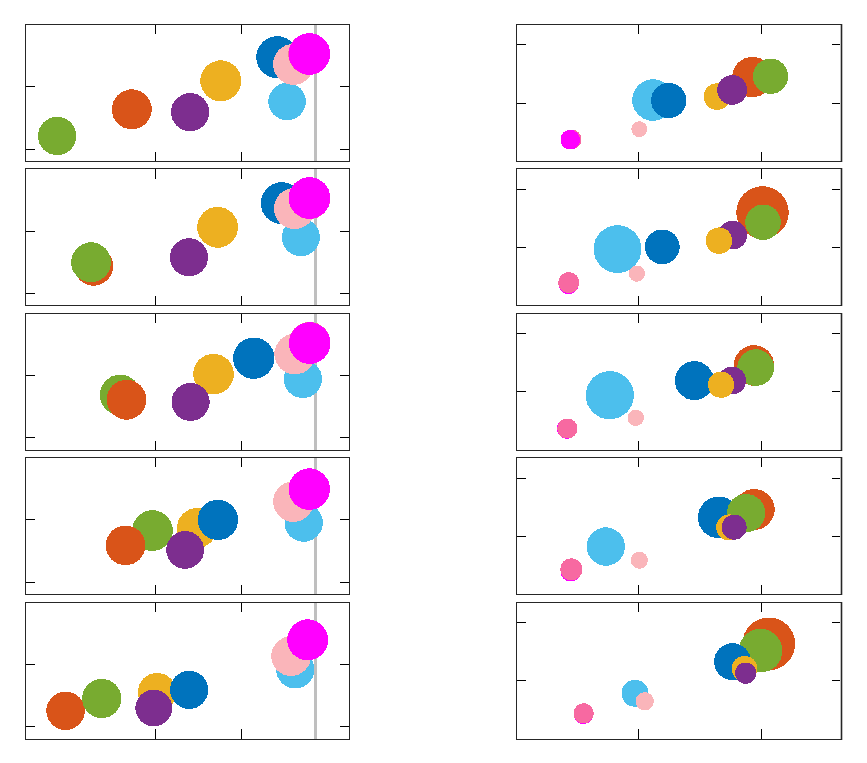
\includegraphics{./figures/parts/02/chapters/04/sections/05//pose_improvement_circles_sm5}}%
    \gplfronttext
  \end{picture}%
\endgroup
